\hypertarget{_matrix_8cpp}{}\section{Visual\+Impro/\+Matrix.cpp File Reference}
\label{_matrix_8cpp}\index{Visual\+Impro/\+Matrix.\+cpp@{Visual\+Impro/\+Matrix.\+cpp}}


\mbox{\hyperlink{class_matrix}{Matrix}} object composed by rows and columns.  


{\ttfamily \#include \char`\"{}Matrix.\+hpp\char`\"{}}\newline
Include dependency graph for Matrix.\+cpp\+:
\nopagebreak
\begin{figure}[H]
\begin{center}
\leavevmode
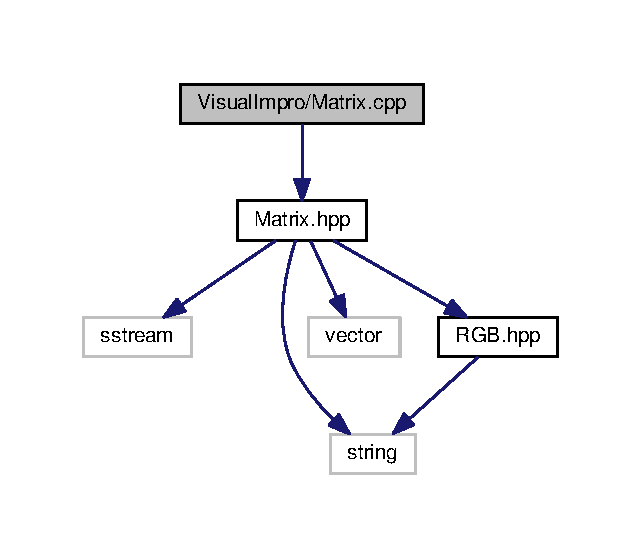
\includegraphics[width=308pt]{_matrix_8cpp__incl}
\end{center}
\end{figure}


\subsection{Detailed Description}
\mbox{\hyperlink{class_matrix}{Matrix}} object composed by rows and columns. 

\begin{DoxyAuthor}{Author}
Alexandre C\+A\+S\+A\+N\+O\+VA--F\+R\+A\+N\+G\+ER, Gauthier L\+A\+R\+M\+A\+R\+Q\+UE, Paul S\+I\+M\+O\+R\+RE, Lucas V\+I\+V\+AS 
\end{DoxyAuthor}
\begin{DoxyDate}{Date}
March 2018
\end{DoxyDate}
The \mbox{\hyperlink{class_matrix}{Matrix}} object is used several times in this program, and replace the vector$<$vector$<$\+T\+Y\+P\+E$>$ $>$ objects. As we process Matrices of signal, this class was clearly needed by the program. 